\chapter{Additional Output Quantities}

\section{Black Hole Accretion}\index{black holes!supermassive}\index{black holes!accretion}\index{black holes!jets}

Properties associated with accretion onto supermassive black holes can be output by setting {\tt blackHoleOutputAccretion}$=${\tt true}. Currently, two additional properties are output for each node when this option is selected:
\begin{description}
\item[{\tt blackHoleAccretionRate}] The rate at which the supermassive black hole is accreting mass in $M_\odot$ Gyr$^{-1}$;
\item[{\tt blackHoleJetPower}] The power being emitted into jets by the black hole/accretion disk system in $M_\odot$ km$^2$ s$^{-2}$ Gyr$^{-1}$.
\end{description}

\section{Cooling Data}\index{cooling}\index{cooling!output}\index{cooling!radius}\index{cooling!rate}

Properties associated with cooling in hot halos can be output by setting {\tt hotHaloOutputCooling}$=${\tt true}. Currently, two additional properties are output for each node when this option is selected:
\begin{description}
\item[{\tt hotHaloCoolingRate}] The rate at which gas is cooling from the halo (assuming no sources of heating) in $M_\odot$ Gyr$^{-1}$;
\item[{\tt hotHaloCoolingRadius}] The characteristic cooling radius in the halo in Mpc.
\end{description}

\section{Density Contrast Data}\index{density contrast}\index{density!contrast}

Properties of nodes at density contrasts other than the virial density can be output by setting {\tt [outputDensityContrastData]}$=${\tt true}. When selected, this output option requires that a list of density contrasts, $\Delta$ (defined in units of the mean density of the Universe), be given in the {\tt [outputDensityContrastValues]} input parameter. For each specified density contrast, two properties are output for each node: {\tt nodeRadius}$\Delta$ and {\tt nodeMass}$\Delta$ which give the radius enclosing a mean density contrast of $\Delta$ and the mass enclosed within that radius. The parameter {\tt [outputDensityContrastDataDarkOnly]} controls whether density contrasts are measured for total mass ({\tt false}) or dark matter mass only ({\tt true}). In the latter case, density contrasts are defined relative to the mean dark matter density of the Universe.

\section{Descendent Node Index}\index{descendent node}\index{node!descendent}

By setting {\tt [outputDescendentIndices]}$=${\tt true} the index of the node containing the galaxy to which each current galaxy will belong at the next output time (i.e. the \gls{forwardDescendent}) will be written to the output file. To clarify, this will be the index of the node into which the galaxy descends, or the index of a node with which it merges prior to the next output time (and if that node merges with another, the index will be of that node and so on).

Note that, to operate correctly, information about which node a given node may merge with (and when this merger will happen) must be available. This is typically available in merger trees read from file providing {\tt [treeNodeMethodSatelliteOrbit]} and {\tt [mergerTreeReadPresetMergerTimes]} are both set to {\tt true}. When using randomly assigned satellite orbits and merger times, information on when merging occurs does not exist until a node becomes a satellite. Thus, if the node becomes a satellite after the current output, but before the next output, there is no way to know which node it will belong to at the next output (in such cases, the fallback assumption is no merging).

\section{Half-Light Radii Data}\index{mass profile!half-light radius}\index{half-light radius}

Half-light radii and masses enclosed within them can be output by setting {\tt [outputHalfLightData]}$=${\tt true}. When selected the half-light radius in each specified luminosity band is output as {\tt [halfLightRadius\{luminosityID\}]} (in Mpc), where {\tt\{luminosityID\}} is the usual luminosity identifier suffix, and the total (dark + baryonic) mass within that radius is output as {\tt [halfLightMass\{luminosityID\}]} (in $M_\odot$).

\section{Halo Model Quantities}\label{sec:HaloModelOutput}\index{halo model}\index{clustering!halo model}

The following quantities related to galaxy clustering are output if {\tt [outputHaloModelData]} is set to true:
\begin{description}
 \item [{\tt nodeBias}] The large scale, lineary theory bias for each node. For satellite nodes, this corresponds to the bias of their host halo;
 \item [{\tt isolatedHostIndex}] The index of the isolated node in which this node lives. This is identical to {\tt nodeIndex} for non-satellite nodes.
\end{description}
In addition to these quantities output for each node, setting {\tt [outputHaloModelData]}$=${\tt true} causes the creation of a {\tt haloModel} group in the \glc\ output file. This group contains the following:
\begin{description}
 \item [{\tt wavenumber}] A dataset giving the wavenumbers (in units of Mpc$^{-1}$) at which all output power spectra are tabulated. The minimum and maximum wavenumbers to tabulate are determined by the {\tt [haloModelWavenumberMinimum]} and {\tt [haloModelWavenumberMaximum]} parameters respectively, while the number of points to tabulate in each decade of wavenumber is determined by the {\tt [haloModelWavenumberPointsPerDecade]} parameter.
 \item [{\tt powerSpectrum}] A dataset giving the linear theory power spectrum (in units of Mpc$^3$ normalized to $z=0$ at each wavenumber specified in the {\tt wavenumber} dataset.
 \item [{\tt Output\{i\}/mergerTree\{j\}/fourierProfile\{k\}}] A dataset giving the Fourier transform of the dark matter halo density profile (dimensionless and normalized to unity at small wavenumber) for the node with index {\tt k} in merger tree with index {\tt j} at output number {\tt i}. Profiles are written only for nodes which are isolated, and are tabulated at the wavenumbers given in the {\tt wavenumber} group. Note that wavenumbers are assumed to be comoving.
\end{description}
Finally, each numbered output group is given two additional attributes, {\tt linearGrowthFactor} and {\tt linearGrowthFactorLogDerivative} which give the growth factor, $D$, and its logarithmic derivative, $\d \ln D / \d \ln a$ at the output time.

The information output can be used to construct galaxy power spectra and correlation functions (see \S\ref{sec:ClusteringHaloModel} for example).

\section{Lightcone Coordinates}\label{sec:OutputLightcone}\index{lightcones}

The position (and velocity and redshift) of a galaxy within a lightcone will automatically be output if the {\tt lightcone} output filter is active (see \S\ref{sec:OutputFilters}). In such cases, the following properties will be output for all galaxies:
\begin{description}
 \item [{\tt lightconePositionX}] Position of the galaxy (in comoving Mpc) along the radial direction of the lightcone;
 \item [{\tt lightconePositionY}] Position of the galaxy (in comoving Mpc) along the 1$^{\rm st}$ angular direction of the lightcone;
 \item [{\tt lightconePositionZ}] Position of the galaxy (in comoving Mpc) along the 2$^{\rm nd}$ angular direction of the lightcone;
 \item [{\tt lightconeVelocityX}] Velocity of the galaxy (in km/s) along the radial direction of the lightcone;
 \item [{\tt lightconeVelocityY}] Velocity of the galaxy (in km/s) along the 1$^{\rm st}$ angular direction of the lightcone;
 \item [{\tt lightconeVelocityZ}] Velocity of the galaxy (in km/s) along the 2$^{\rm nd}$ angular direction of the lightcone;
 \item [{\tt lightconeRedshift}] Redshift of the galaxy in the lightcone\footnote{Note that this will not, in general, be precisely the same as the redshift corresponding to the output time.};
 \item [{\tt angularWeight}] The mean number density of this galaxy per unit area on the sky (in degrees$^{-2}$).
\end{description}
If active, the geometry of the lightcone must be specified in an XML file, the name of which must be specified using the {\tt [filterLightconeGeometryFileName]} input parameter. The XML file should have the following structure:
\begin{verbatim}
<geometry>
  <boxLength>500</boxLength>
  <cosmology>
    <parameter>
      <name>omega0</name>
      <value>0.25</value>
    </parameter>
    <parameter>
      <name>lambda0</name>
      <value>0.75</value>
    </parameter>
    <parameter>
      <name>H0</name>
      <value>70</value>
    </parameter>
  </cosmology>
  <fieldOfView>
    <geometry>square</geometry>
    <length>0.0174532927777778</length>
  </fieldOfView>
  <maximumDistance>6136.78369140625</maximumDistance>
  <origin>
    <coordinate>50</coordinate>
    <coordinate>50</coordinate>
    <coordinate>50</coordinate>
  </origin>
  <outputs>
    <maximumDistance>9606.4736328125</maximumDistance>
    <maximumDistance>9470.22194965342</maximumDistance>
    .
    .
    .
    <minimumDistance>9470.22194965342</minimumDistance>
    <minimumDistance>9160.59527164611</minimumDistance>
    .
    .
    .
    .
    <redshift>127</redshift>
    <redshift>79.997894</redshift>
    .
    .
    .
  </outputs>
  <unitVector1>
    <coordinate>0.307692307692308</coordinate>
    <coordinate>0.230769230769231</coordinate>
    <coordinate>0.923076923076923</coordinate>
  </unitVector1>
  <unitVector2>
    <coordinate>0</coordinate>
    <coordinate>0.923076923076923</coordinate>
    <coordinate>-0.230769230769231</coordinate>
  </unitVector2>
  <unitVector3>
    <coordinate>-0.905325443786982</coordinate>
    <coordinate>0.0710059171597633</coordinate>
    <coordinate>0.284023668639053</coordinate>
  </unitVector3>
  <units>
    <length>
      <hubbleExponent>-1</hubbleExponent>
      <unitsInSI>3.08568025e+22</unitsInSI>
    </length>
  </units>
</geometry>
\end{verbatim}
The {\tt boxLength} element should give the length of the simulation box (the box will be replicated to span the volume covered by the lightcone), while the {\tt maximumDistance} element should specify the largest distance in the lightcone to be considered. The {\tt fieldOfView} element must specify the geometry of the field of view. Currently, the only allowed value for the {\tt geometry} of the {\tt fieldOfView} element is {\tt square}, in which case the {\tt length} element of {\tt fieldOfView} should give the length of the side of the square field of view in radians. The {\tt origin} element must contain the $x$, $y$, $z$ {\tt coordinate}s of the origin of the lightcone within the simulation box, while the {\tt unitVectorX} elements must give unit vectors which point along the lightcone (for {\tt X}$=1$, and in the two directions perpendicular to the lightcone (for {\tt X}$=2$ and 3). The {\tt outputs} element contains lists of properties corresponding to the outputs to be used for building the lightcone.
 The {\tt redshift} subelements must list the redshifts of available outputs (in order of decreasing redshift) while the {\tt minimumDistance} and {\tt maximumDistance} elements must give the minimum and maximum comoving distance that should be considered to be associated with each given output redshift. The {\tt units/length} element must specify the units used for lengths, with {\tt unitsInSI} giving the length unit in SI units and {\tt hubbleExponent} giving the exponent of $h$ that appears in the length unit. Finally, the optional {\tt cosmology} element may give cosmological parameters relevant to this lightcone in standard \glc\ format.

\section{Main Branch Evolution}\index{main branch!evolution}\index{evolution!main branch}

The evolution of main branch galaxies can be recorded by setting {\tt [timestepRecordEvolution]}$=${\tt true}. When set, the evolution of each main branch galaxy will be recorded at a set of {\tt [timestepRecordEvolutionSteps]} timesteps spaced logarithmically in cosmic time between {\tt [timestepRecordEvolutionBegin]} and \newline {\tt [timestepRecordEvolutionEnd]}. 

This recorded evolution will be written to the group {\tt mainProgenitorEvolution} in the \glc\ output file. Within that group two datasets, {\tt time} and {\tt expansionFactor}, give the times and expansion factors at which evolution was recorded. Then for each merger tree two datasets, {\tt stellarMass<N>} and {\tt totalMass<N>} (where {\tt <N>} is the merger tree index), give the stellar and total baryonic mass of the main branch progenitor at each timestep.

\section{Main Branch Status}\index{merger trees!main branch}

The status of each node with respect to the main branch of its merger tree can be output by setting {\tt [outputMainBranchStatus]}$=${\tt true}. When set, the status will be output as {\tt nodeIsOnMainBranch}, with a value of 1 indicating that the node is a primary progenitor of the final halo (i.e. is on the main branch of the tree) and a value of 0 indicating that it is not.

\section{Mass Profile Data}\index{mass profile}

Masses enclosed within specific radii can be output by setting {\tt [outputMassProfileData]}$=${\tt true}. When selected, this output option requires that a list of radii, $r$ (in Mpc), be given in the {\tt [outputMassProfileRadii]} input parameter. For each specified radius, the total (dark + baryonic) mass will be output as {\tt massProfile}$r$.

\section{Merger Tree Links and Node Isolation}\index{merger tree!links}\index{galaxies!satellite}\index{galaxies!central}\index{nodes!isolated}\index{nodes!substructure}

The following properties are output to permit the merger tree structure to be recovered:
\begin{description}
 \item [{\tt nodeIndex}] A unique (within a tree) integer index identifying the node;
 \item [{\tt childIndex}] The index of this node's primary child node (or $-1$ if it has no child);
 \item [{\tt parentIndex}] The index of this node's parent node (or $-1$ if it has no parent);
 \item [{\tt siblingIndex}] The index of this node's sibling node (or $-1$ if it has no sibling);
 \item [{\tt satelliteIndex}] The index of this node's first satellite node (or $-1$ if it has no satellites);
 \item [{\tt nodeIsIsolated}] Will be $0$ for a node which is a subhalo inside some other node (i.e. a satellite galaxy\index{satellite galaxies!identifying}) or $1$ for a node that is an isolated halo (i.e. a central galaxy\index{central galaxies!identifying}).
\end{description}

The {\tt nodeIndex} property corresponds by default to the index of the node in the original merger tree. This means that as a galaxy evovles through the tree and, in particular, gets promoted into a new halo the index associated with a galaxy will change. This is useful to identify where the galaxy resides in the original (unevolved) tree structure, but does not allow galaxies to be traced from one output to the next using their {\tt nodeIndex} value. By setting {\tt [nodePromotionIndexShift]}$=${\tt true} this behavior can be changed such that the value of {\tt nodeIndex} will reflect the index of the earliest progenitor node along the main branch of the current node. As such, this index will remain the same for a given galaxy during its evolution\index{galaxies!tracing through outputs}\index{galaxies!indices}\index{nodes!indices}\index{indices!nodes}\index{indices!galaxies}. These two alternative algorithms for propagating node indices are illustrated in Figure~\ref{fig:NodePromotionIndexAlgorithms}.

\begin{figure}
 \begin{center}
 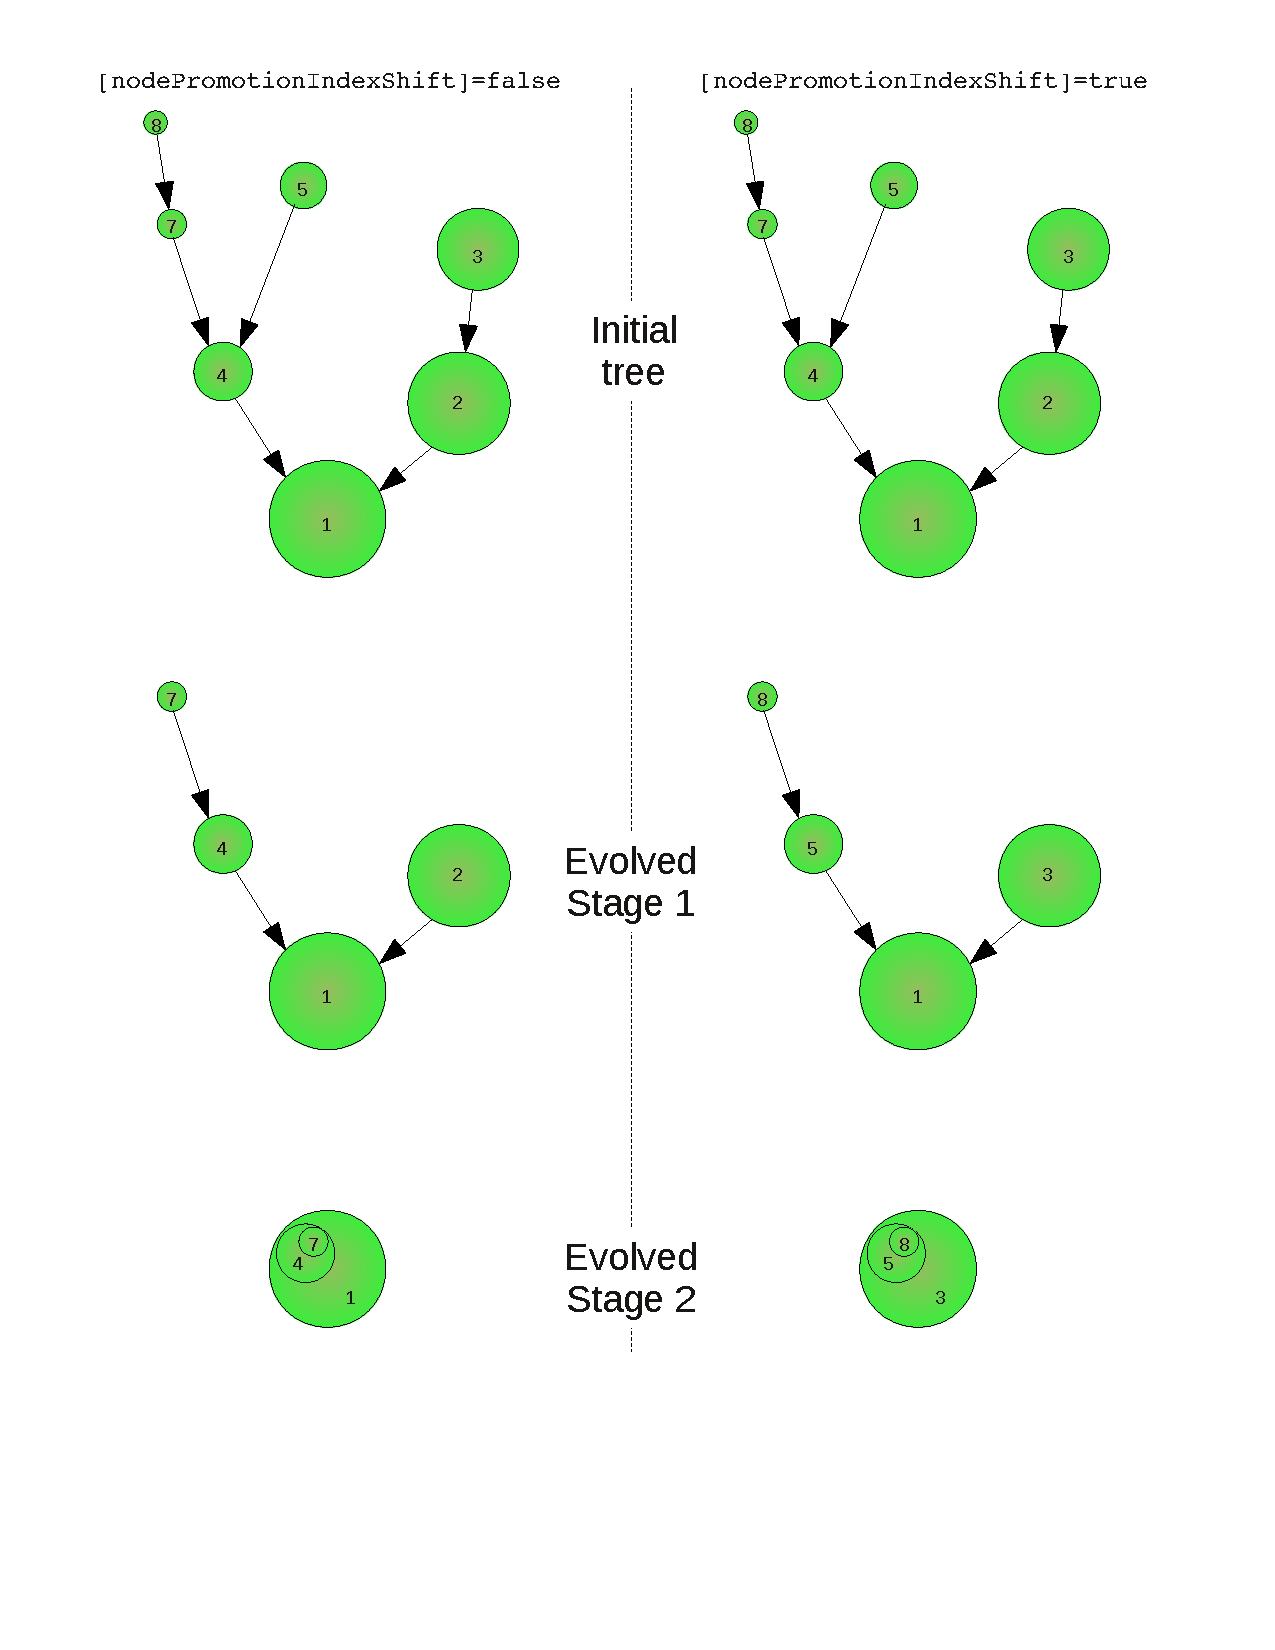
\includegraphics[width=140mm]{Diagrams/NodePromotionIndices.pdf}
 \end{center}
 \caption{Illustration of options for the propagation of node indices during node promotion events. Two identical trees (top row) are evolved with {\tt [nodePromotionIndexShift]}$=${\tt false} (left column) and {\tt [nodePromotionIndexShift]}$=${\tt true} (right column). The middle and lower rows indicate the resulting node indices after two stages of tree evolution.}
 \label{fig:NodePromotionIndexAlgorithms}
\end{figure}

\section{Merger Tree Data for Rendering}\index{merger tree!rendering}

Data on the structure of a merger tree and its halos useful for rendering the tree as a 3-D structure can be output using the \hyperlink{merger_trees.render.F90:merger_trees_render}{\tt Merger\_Trees\_Render} module. Calling \hyperlink{merger_trees.render.F90:merger_trees_render:merger_trees_render_dump}{\tt Merger\_Trees\_Render\_Dump} with a tree as the only argument will cause the tree structure will be dumped to a file named {\tt render\_$\langle$treeIndex$\rangle$\_$\langle$outputIndex$\rangle$.hdf5} where $\langle${\tt treeIndex}$\rangle$ is the index of the tree and $\langle${\tt outputIndex}$\rangle$ is an incremental counter that tracks the number of outputs for this tree. The output is a simple HDF5 file containing the following datasets:
\begin{description}
 \item [{\tt nodeIndex}] Index of the node;
 \item [{\tt parentIndex}] Index of the parent node;
 \item [{\tt childIndex}] Index of the child node;
 \item [{\tt time}] Time of the node;
 \item [{\tt expansionFactor}] Corresponding expansion factor;
 \item [{\tt radiusVirial}] Virial radius of the node;
 \item [{\tt position}] $(x,y,z)$ position of the node.
\end{description}

\section{Merger Tree Structure}\index{merger tree!structure}

The structure of each merger tree can optionally be dumped to a file suitable for post-processing with \href{http://www.graphviz.org/}{\sc dot} after every step of evolution. To request this output set {\tt [mergerTreesDumpStructure]}$=${\tt true}. After each evolution step the tree structure will be dumped to a file named {\tt mergerTreeDump:$\langle$treeIndex$\rangle$:$\langle$outputIndex$\rangle$.gv} where $\langle${\tt treeIndex}$\rangle$ is the index of the tree and $\langle${\tt outputIndex}$\rangle$ is an incremental counter that tracks the number of outputs for this tree. These files can be processed with \href{http://www.graphviz.org/}{\sc dot} to produce a diagram of the tree structure. The node currently being evolved will be highlighted in green. This output option makes use of the \hyperlink{objects.merger_trees.dump.F90:merger_trees_dump}{\tt Merger\_Trees\_Dump} module to create the outputs.

\section{Most Massive Progenitor}

Setting {\tt [outputMostMassiveProgenitor]}$=${\tt true} causes the property {\tt isMostMassiveProgenitor} to be output. This propert will be $1$ for the most massive progenitor node in a tree at each output time and $0$ for all other nodes.

\section{Star Formation Rates}\index{star formation rate!outputting}\index{outputs!star formation rate}

By default the star formation rate in each galaxy is \emph{not} output. However, setting {\tt [diskOutputStarFormationRate]} to true will cause the current star formation rate in the disk of each galaxy to be output as {\tt diskStarFormationRate} (in units of $M_\odot$/Gyr). The {\tt [spheroidOutputStarFormationRate]} has the same effect for the spheroid component.

\section{Virial Quantities}\index{virial}

The following quantities related to the virialized region of each node are output if {\tt outputVirialData} is set to true:
\begin{description}
 \item [{\tt nodeVirialRadius}] The virial radius (following whatever definition of virial overdensity was selected in \glc) in units of Mpc;
 \item [{\tt nodeVirialVelocity}] The circular velocity at the virial radius (in km/s).
\end{description}
